\section{Hash Functions and Associative Caches}
\label{sec:Problem}

As noted above, many-core architectures typically have several processors on
chip, and these processors will have their own caches and routing logic to
connect them to other processors.  They might even have other peripherals
associated such as floating point units.  An example arrangement of processors
in a many-core system, as well as a view of what a single tile looks like, are
shown in Figures \ref{Fig:piton_arch} and \ref{Fig:piton_tile}, both taken from
the OpenPiton architecture \cite{openpiton}.

\begin{figure}[h]
  \centering
  \begin{minipage}[b]{0.4\textwidth}
    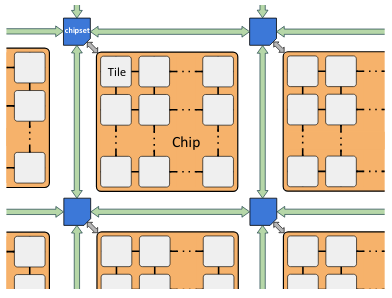
\includegraphics[width=\textwidth]{figures/piton_arch.png}
    \caption{OpenPiton architecture}
    \label{Fig:piton_arch}
  \end{minipage}
  \hfill
  \begin{minipage}[b]{0.4\textwidth}
    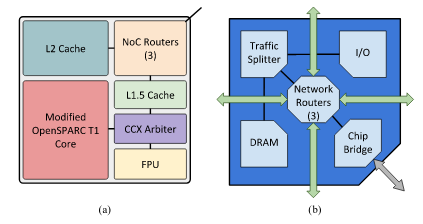
\includegraphics[width=\textwidth]{figures/piton_tile_and_chipset.png}
    \caption{OpenPiton tile and chipset}
    \label{Fig:piton_tile}
  \end{minipage}
\end{figure}


In a many-core architecture with several identically sized caches, such as the
OpenPiton system, the problem of finding the specific data associated with a
memory address can be broken into two phases.  In the first phase a memory
address is homed to a cache on a specific tile.  In the second phase the memory
address is parsed to determine the exact line of the cache where the relevant
data is stored.  The first phase is the subject of our investigations, and so we
will canvas the second phase now, before diving into the details of the first
phase.

The second phase of retrieving a cache line is accomplished by breaking down the
address into subsets, with each subset of bits referring to a different level of
the memory hierarchy.  For instance, in Figure \ref{Fig:memory_addr}, we can see
such a division.  With tag and index, bits, we specify narrower regions of the
cache, until the offset picks exactly which cache line holds that specific
address.

\begin{figure}[h]
  \centering
  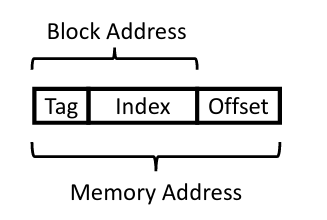
\includegraphics[scale=0.4]{figures/memory_addr.png}
  \caption{A memory address}
  \label{Fig:memory_addr}
\end{figure}

In the first phase, because the data associated with the address can be stored
in any cache, we are simply trying to distribute the addresses evenly across chips.  This prevents traffic jams on the network interconnects between
chips and gives all memory equal access times.  To accomplish this, hardware
architects employ hash functions, which are mappings from objects (the memory
addresses) to identifiers, or hashes (the tiles).  The mappings are
deterministic, in that they compute the same hash for a key every time, are fast
to compute (comprising of only bitvector operations), and evenly distribute the
keys among the available hashes.

This scheme is inflexible however, if the sizes of the caches change.  This is
due to a fact about modern cache design, namely, associativity.  Associativity
describes how efficiently we can place data into the cache.  In
fully-associative caches, data may be placed anywhere.  In a
non-fully-associative, or ``direct-mapped'' cache, data is placed into the cache
according to a simple scheme that possibly ejects memory already in the cache.
Because of this, direct-mapped caches tend to show poor overall utilization,
while fully-associative caches show increased utilization, and therefore suggest
more efficient use of silicon.

We can see that for a many-core architecture with caches that are at least
partially associative, using a traditional hash function will result in overall
worse utilization.  Because memory addresses are mapped uniformly to all caches,
larger caches will have proportionately fewer lines inhabited, and smaller
caches will have all of their lines inhabited.  To address this mismatch, we
will investigate strategies for mapping memory addresses into caches
proportionate to their sizes, thus maintaining high utilization across caches.

